\documentclass{udpreport}
\title{Sockets}
\author{Integrantes: Francisca Carrrasco, Ignacio López, Nicolás Ramírez.\\Profesor: José Pérez
\\Ayudante: Alexis Inzunza}
\date{Junio de 2017}
\usepackage{graphicx}
\graphicspath{ {Imagenes/} }
\udpschool{Escuela de Informática y Telecomunicaciones}

\begin{document}
\maketitle
\tableofcontents
\listoffigures
 
\chapter{Actividades}
	\section{Actividad 1:}
	    Se creará un algoritmo en el programa "Python",en el cual se importará la librería "socket", la que se basa en la API "Sockets de Berkeley", que es una implementación de los sockets.\\\\
		{\large \bf{Cliente y Servidor: }}
		\begin{figure}[h]
    \centering
    \includegraphics[width=11.7cm, height=6.5cm]{servidor.png}
    \caption{Servidor}
    \includegraphics[width=11.7cm, height=6.5cm]{cliente.png}
    \caption{Cliente}
    \end{figure}
    \newpage
   

	
  
	\section{Actividad 2:}
        Utilizando Wireshark, se analizará el tráfico de información.
        \\\\
	{\large \bf{Wireshark: }}\\ 
	\begin{figure}[h]
    \centering
    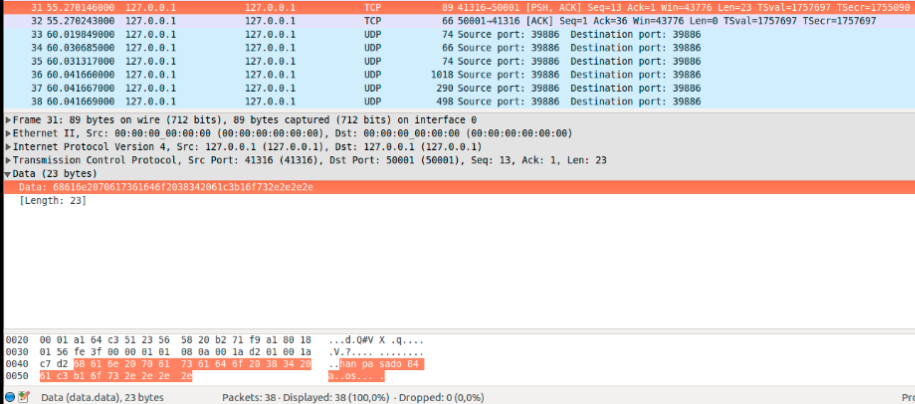
\includegraphics[width=18cm, height=10cm]{capturaalacapturaalacaptura.png}
    \caption{Wireshark}
    \end{figure}
    \newpage

	\chapter{Preguntas propuestas:}	\\
	\begin{enumerate}
	    \item Utilizando la información obtenida en la actividad 2, explique el funcionamiento del envío y recepción
    de información para su algoritmo, respondiendo a las interrogantes ¿Qué se envía? ¿Cómo se envía?\\\\
        Con nuestro algoritmo, enviamos mensajes con el protocolo tcp, con el uso de la librería "socket" en Python.
        Como lo que usamos fue el protocolo tcp, se utiliza en protocolo de 3 vías el cual consiste en .\\
        \item ¿Por qué el puerto que muestra el servidor al generar la conexión no es el mismo que el escrito en el
    algoritmo del ciente?\\\\
                       Porque el cliente toma un puerto aleatorio (que esté libre) para poder enviar el mensaje, 
                       ya que en el algoritmo nunca se definió el puerto por el que debía salir.\\ 
                                            
        \item Si usted tuviese que realizar un videojuego con soporte multijugador utilizando sockets ¿Qué protocolo
    utilizaría? ¿Por qué? \\\\  
            El protocolo más adecuado de utilizar sería UDP, ya que en este protocolo es más importante la velocidad 
            que el envío de todos los datos y que el programa no se quede bloqueado (sin poder enviar información).\\
                                          
        \item¿Se puede utilizar cualquier número de puerto para cualquier aplicación? Explique.\\\\
            El número del puerto se puede elegir libremente, siempre y cuando este dentro del rango de 1024-65535,
            ya que del 1-1023(el 0 está reservado, es un valor permitido como puerto origen, se usa si el emisor no espera
            recibir respuesta) se encarga de controlar y asignar la  Autoridad de Números Asignados de Internet(IANA) para 
            los servicios de red del UNIX(telnet, ftp) y si no está ocupado en otro programa.\\
        \newpage

	\end{enumerate}

	
\chapter{Conclusión}
 En esta experiencia pudimos aprender a implementar socket de la librería "socket" en Python, programar un algoritmo que
 ejecutado envie mensajes de un "cliente" a un "servidor", estableciendo el uso de puertos e IP.Así haciendo el uso adecuado
 de los protocolos tcp y udp, sabiendo sus diferencias y el momento adecuado de su uso .\\
 
\begin{thebibliography}{x}
\bibitem{Sockets Python}
\textit{http://victorpando.blogspot.cl/2008/12/programacion-de-sockets-con-python.html}
